%%%%%%%%%%%%%%%%%%%%%%%%%%%%%%%%%%%%%%%%%%%%%%%%%%%%%%%%%%%%%%%%%%%%%%%%%%%%%%%
\section{Flujometrías}

De los resultados de la primer otpimización se obtuvo la geometria de los
puertos y una curva de diferencia de presión contra alzada a diferentes
velocidades de giro del motor, con el fin de identificar los puntos de mayor
interés para realizar las flujometrías.

% inicialmente se propusieron un total de XXX flujometŕias, sin embargo algunas
% combinaciones de $\l_{v}, \Delta P$ no se pudieron ejecutar hasta la
% convergencia del flujo másico, por lo que se redujo la cantidad de flujometrías
% final a xxx flujometrías, xxx para el puerto de admisión y xxx para el puerto
% de escape, el par  se detalla en la figura XXX y tabla xxx.

Los pares $(l_{v}, \Delta P)$ seleccionados se detallan en las
figuras~\ref{fig:delta_p_admision} y~\ref{fig:delta_p_escape}, en estos puntos
se busca estimar el coeficiente de descarga para generar el mapa de
funcionamiento del puerto.

\begin{figure}[h]
  \centering
  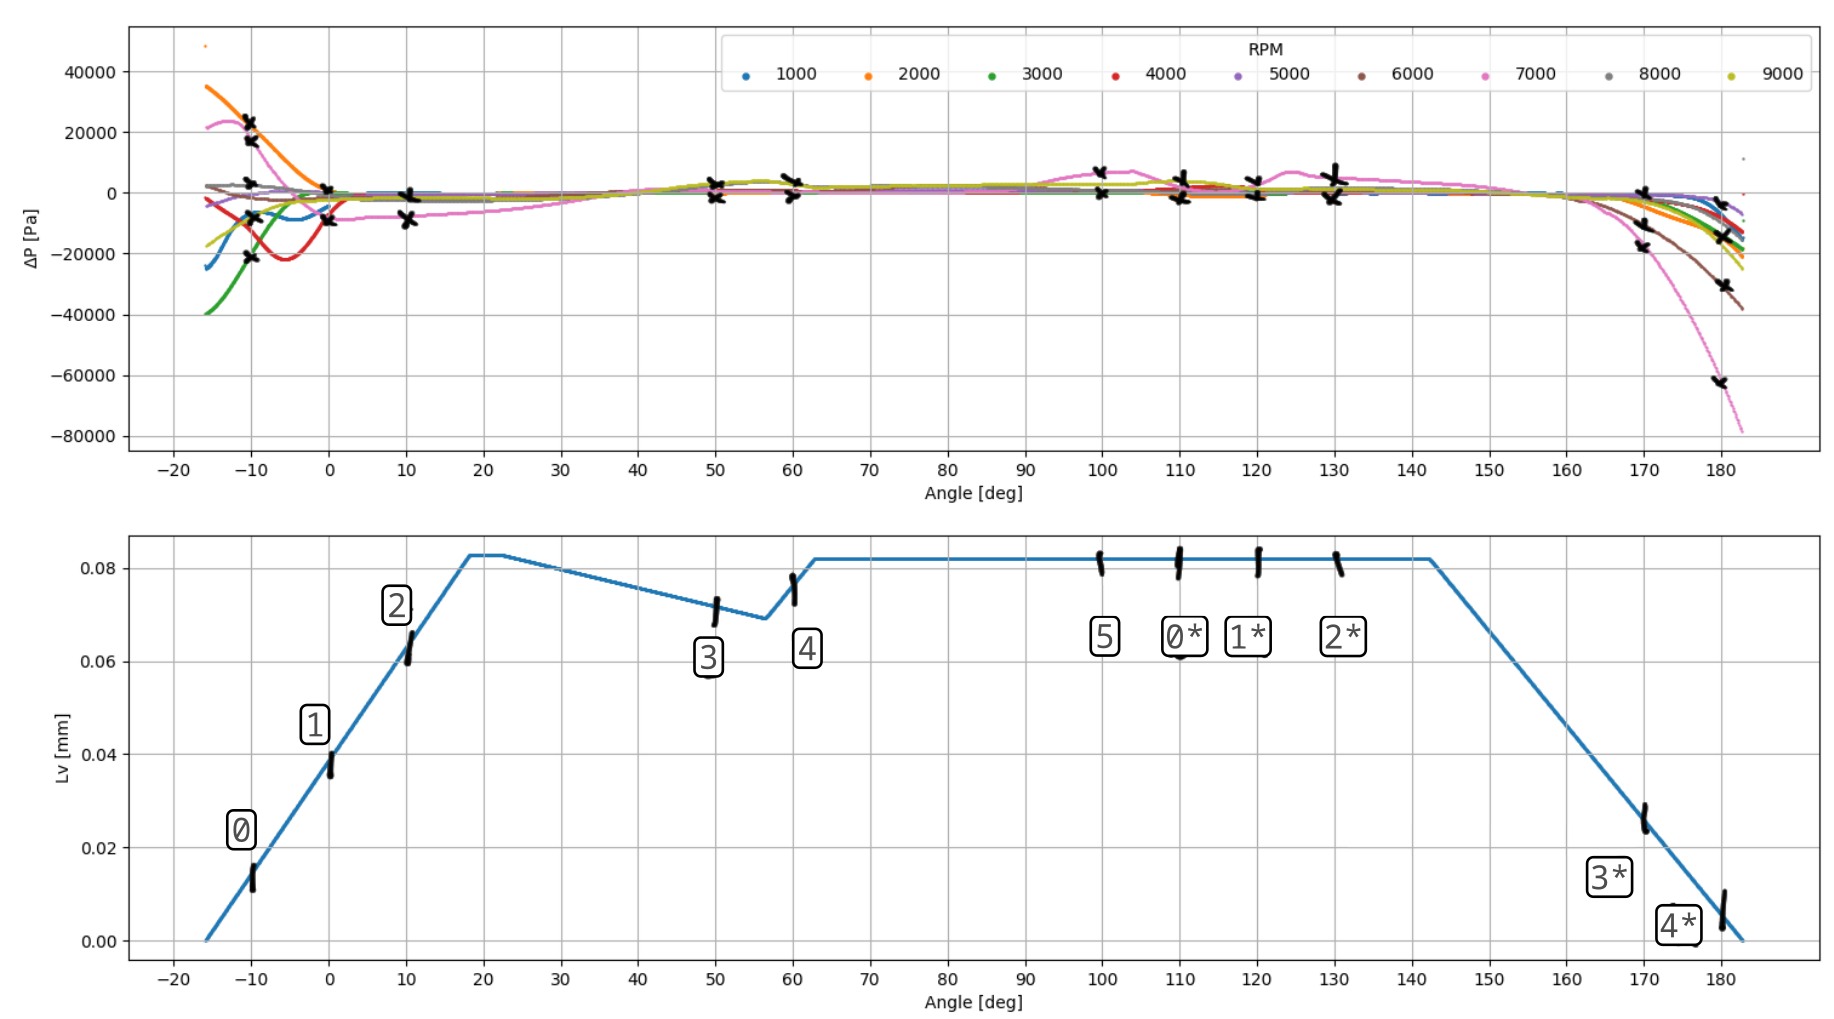
\includegraphics[width=\textwidth]{flujometrias/admision_delta_p_anot.png}
  \caption{Flujometrías puerto de admisión}\label{fig:delta_p_admision}
\end{figure}

\begin{figure}[h]
  \centering
  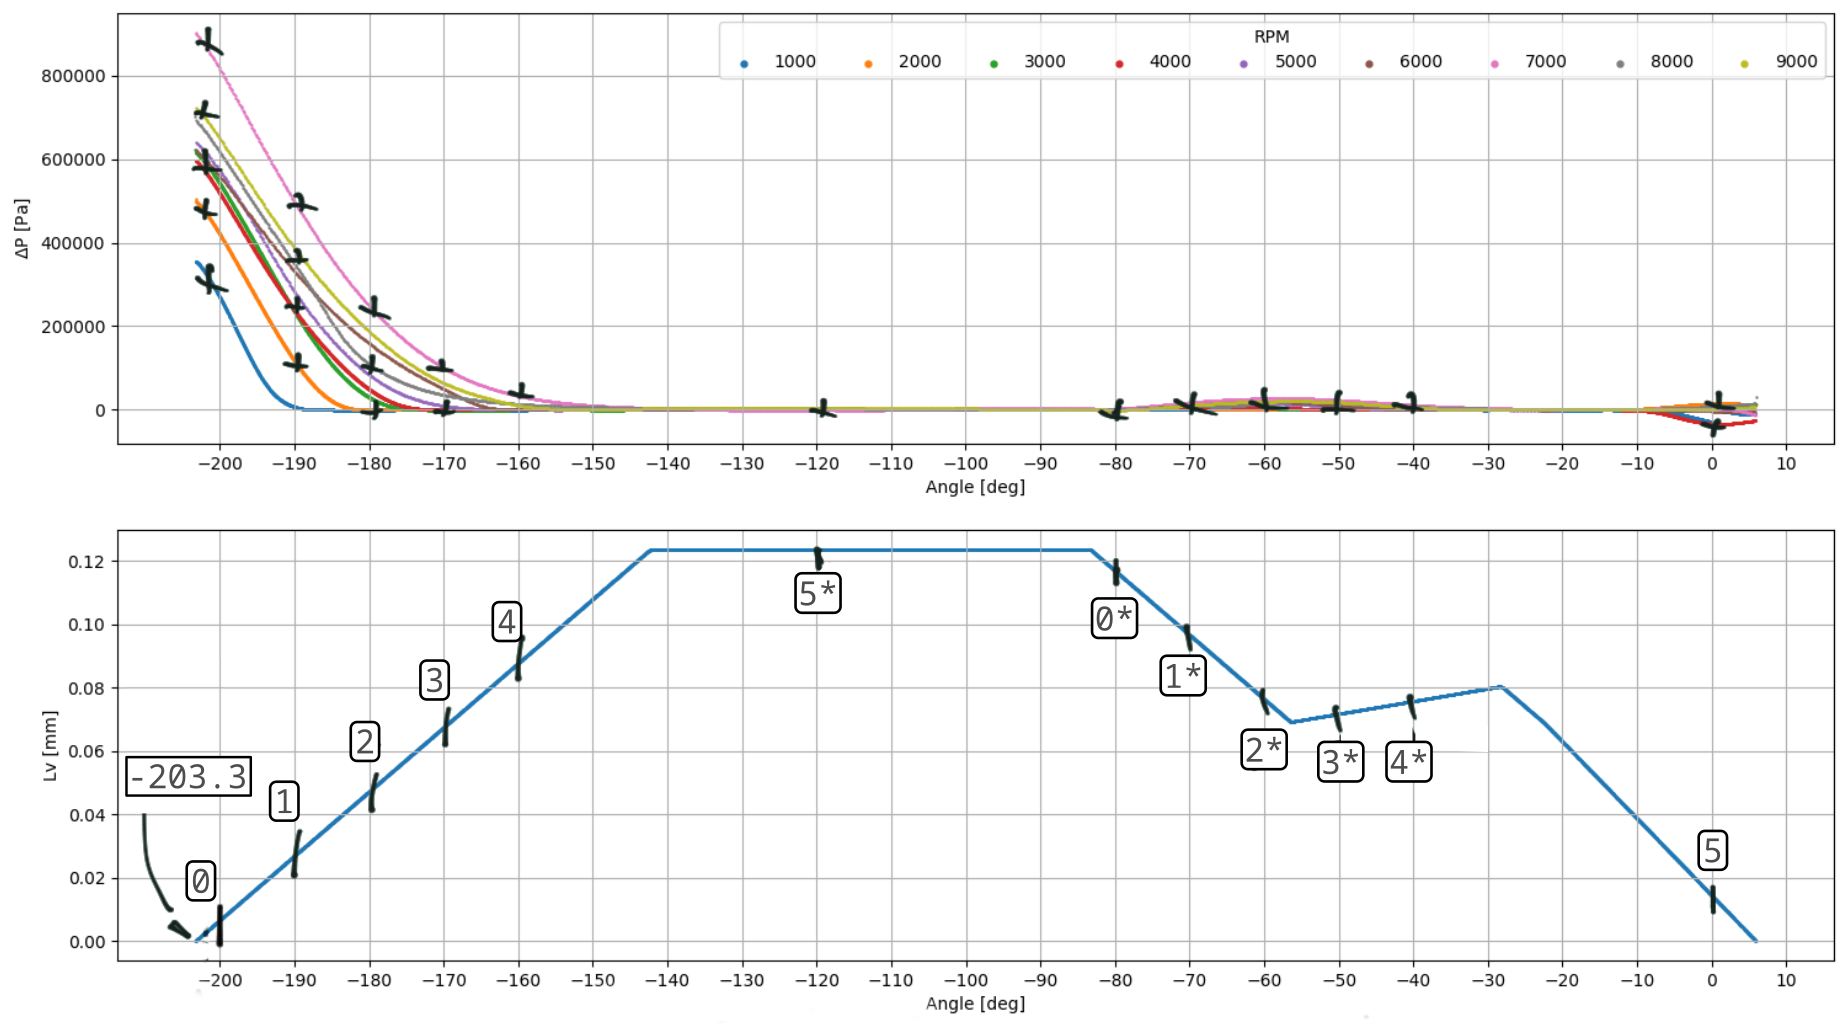
\includegraphics[width=\textwidth]{flujometrias/escape_delta_p_anot.png}
  \caption{Flujometrías puerto de escape}\label{fig:delta_p_escape}
\end{figure}

De las 51 flujometŕias propuestas se realizaron un total de 36 simulaciones las
cuales devoliveron un 56 puntos de valores de $C_{D}$.

\begin{table}[ht]
  \centering
  \begin{tabular}{cccccc}\toprule
    GRA/RPM & 1000 & 2000 & 3000 & 7000 & 9000 \\ \midrule
    0       & -    & X    & -    & X    & - \\
    10      & -    & -    & -    & X    & - \\
    50      & -    & -    & X    & X    & X \\
    100     & X    & -    & -    & X    & - \\
    590     & X    & X    & X    & -    & - \\ \bottomrule
  \end{tabular}
  \caption{Flujometrías puerto de admisión}\label{tab:flujometrias_admision}
\end{table}


\begin{table}[ht]
  \centering
  \begin{tabular}{cccccccc}\toprule
    GRA/RPM & 1000 & 2000 & 3000 & 4000 & 7000 & 8000 & 9000 \\ \midrule
    405     & X    & X    & -    & -    & X    & -    & X \\
    410     & -    & X    & -    & X    & X    & X    & - \\
    420     & -    & -    & -    & X    & -    & X    & - \\
    430     & -    & X    & -    & -    & -    & -    & - \\
    440     & X    & -    & -    & -    & X    & -    & X \\
    500     & -    & -    & X    & -    & X    & X    & - \\ \bottomrule
  \end{tabular}
  \caption{Flujometrías puerto de escape}\label{tab:flujometrias_escape}
\end{table}

Algunas flujometŕias se realizaron en tres etapas, partiendo de una malla gruesa
con celdas de 15mm de tamaño inicial, culminando en celdas de 5mm.
%
En otros se realizó directamente la flujometría con mallas base de 5mm de lado.

En general se simuló alrededor de 0.2 segundos de flujo lo cual fue suficiente
en muchos casos para que se alcance un estado estacionario del flujo, como se ve
en la figura~\ref{fig:flujoemtrias_1_a} y~\ref{fig:flujoemtrias_1_b}.
%
En la primera se presenta el desarrollo del flujo másico para el puerto de
admisión con el cigüeñl en $\theta=10^{\circ}$, para esta posición hay solape de
cámaras por lo que se tienen dos flujos másico, el gráfico de la izquierda
corresponde a una cámara de combustión con $\theta=10^{\circ}$ y la próxima
corresponde a $\theta=130^{\circ}$.
%
En ámbos gráficos se ve una línea de color anaranjado sobre el final de la
simulación, esta representa la poricón de datos que se seleccionó para calcular
el caudal másico.

\begin{figure}[ht]
  \centering
  \begin{subfigure}{\textwidth}
    \centering
    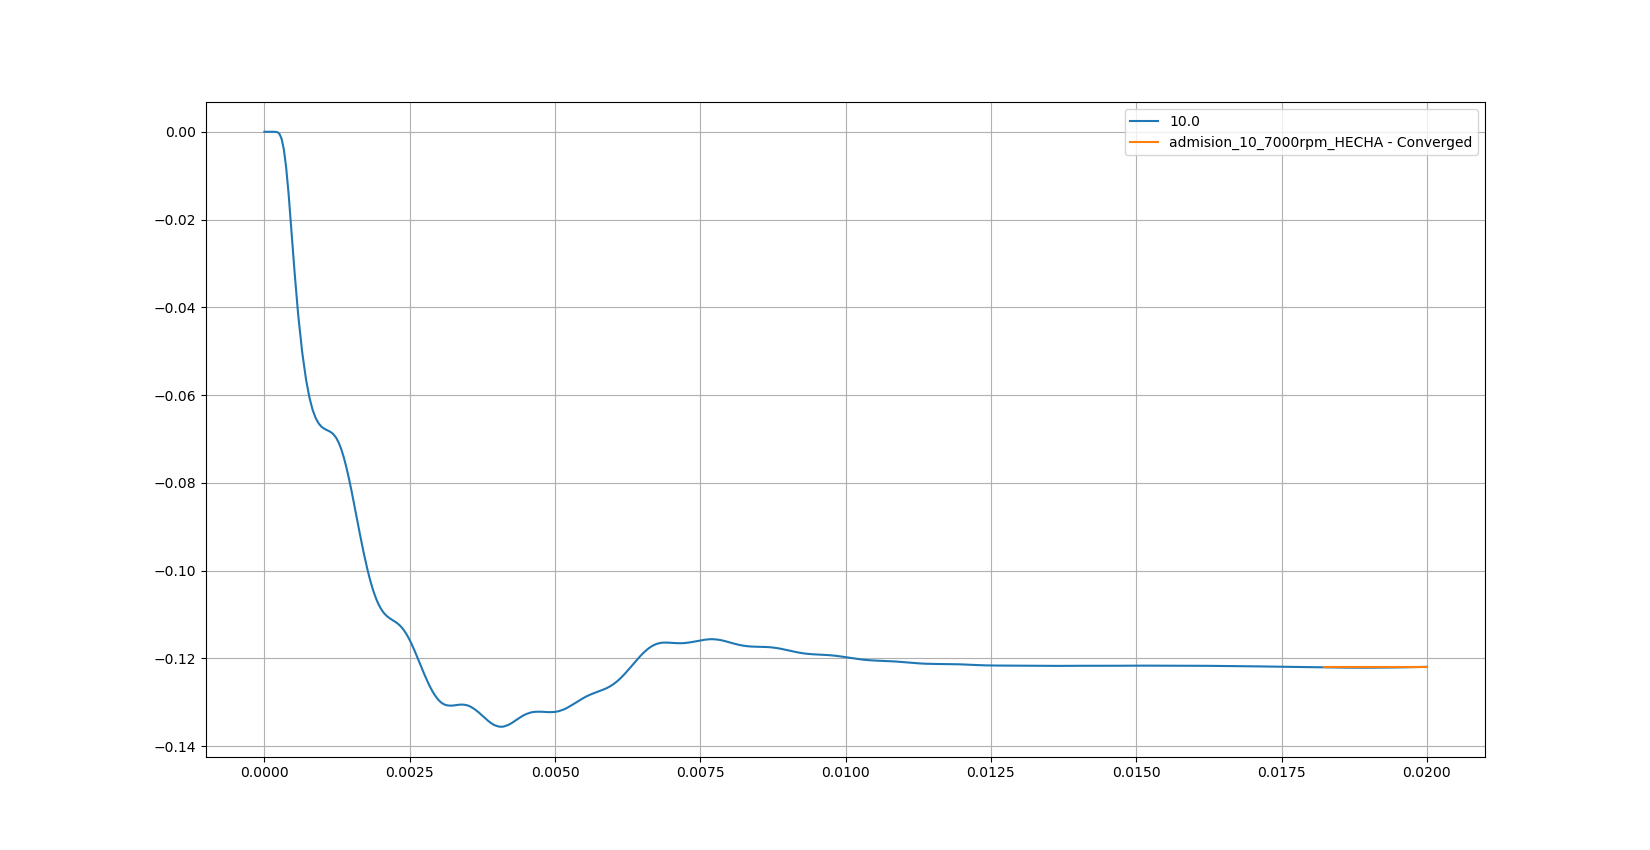
\includegraphics[width=\textwidth]{flujometrias/admision_SFV_10_0.png}
    \caption{Cámara 0 ($\theta=10^{\circ}$)}\label{fig:flujoemtrias_1_a}
  \end{subfigure}
  \hfill
  \begin{subfigure}{\textwidth}
    \centering
    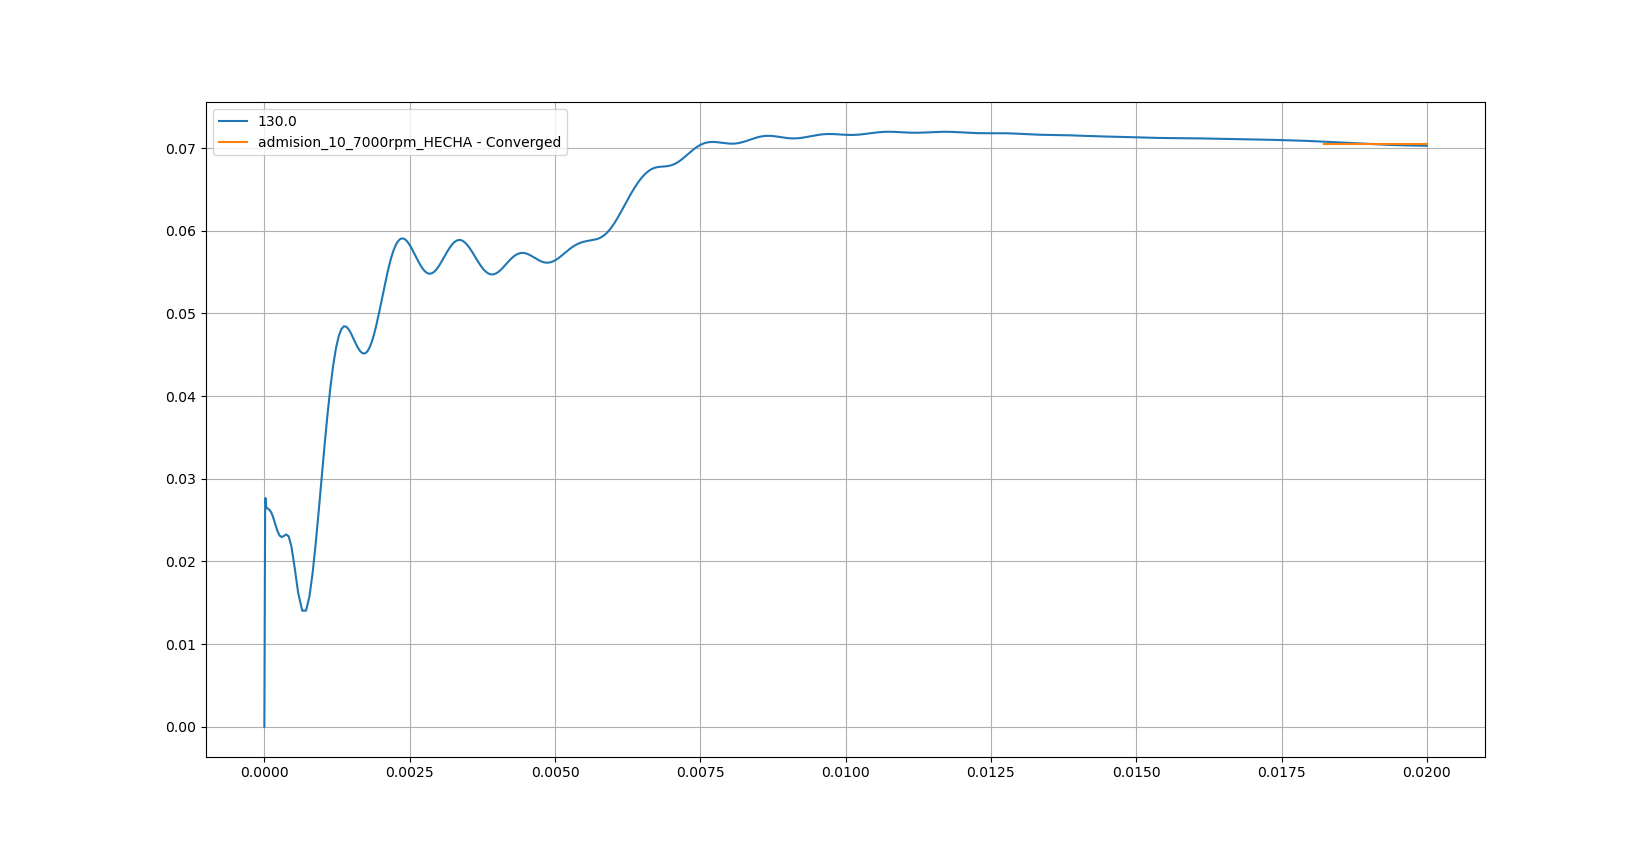
\includegraphics[width=\textwidth]{flujometrias/admision_SFV_130_0.png}
    \caption{Cámara 1 ($\theta=130^{\circ}$)}\label{fig:flujoemtrias_1_b}
  \end{subfigure}
  \caption{Avance de $\dot{m_{f}}$ con tiempo de simulación}\label{fig:flujometrias_1}
\end{figure}



% TODO: esto lo ebería indicar mas abajo, como parte de los detalles que doy
% cuando hable del mapa de coeficiente de descarga obtenido.

% \begin{figure}[ht]
%   \centering
%   \includegraphics[width=\textwidth]{flujometrias/adm_0_2000.png}
%   \caption{Puerto de admisión 0º \@ 2000RPM}\label{fig:adm_0_2000}
% \end{figure}

% \begin{figure}[ht]
%   \centering
%   \includegraphics[width=\textwidth]{flujometrias/adm_100_1000.png}
%   \caption{Puerto de admisión 100º \@ 1000RPM}\label{fig:adm_100_1000}
% \end{figure}

% \begin{figure}[ht]
%   \centering
%   \includegraphics[width=\textwidth]{flujometrias/adm_50_7000.png}
%   \caption{Puerto de admisión 50º \@ 7000RPM}\label{fig:adm_50_7000}
% \end{figure}

Como se mencionó en el apartado~\ref{capitulo:DESARROLLO}, la modificaión
realizada a ICESym para funcionar con un mapa de $C_{D}$ dependiente de dos
variables requiere que los datos de entrada estén distribuidos en una grilla
rectangular.
%
A partir de las flujometrías realizadas se confeccionó el mapa de $C_{D}$, la
totalidad de puntos evaluados se presenta en la tabla~\ref{tab:mapa_cd} en el
adjunto~\ref{adj:mapa_cd}.
%
Los datos obtenidos no forman una grilla rectangular, por lo que se utilizó
un método de suavizado de promedio móvil con $N=2$ para generar dicha grilla, el
resultado se ve en las figuras~\ref{fig:mapa_cd_admision}
y~\ref{fig:mapa_cd_escape}.

\begin{figure}[ht!]
    \centering
    \begin{subfigure}{0.7\textwidth}
        \centering
        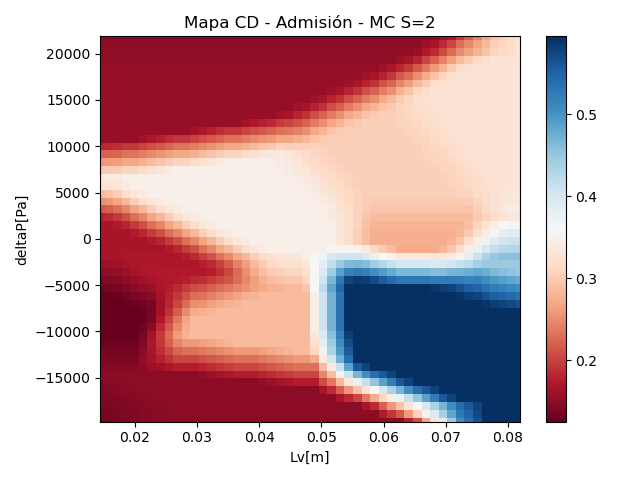
\includegraphics[width=\textwidth]{mapa_cd/mc_s2_mapa_adm.png}
        \caption{Puerto de admisión}\label{fig:mapa_cd_admisión}
    \end{subfigure}
    \hfill
    \begin{subfigure}{0.7\textwidth}
        \centering
        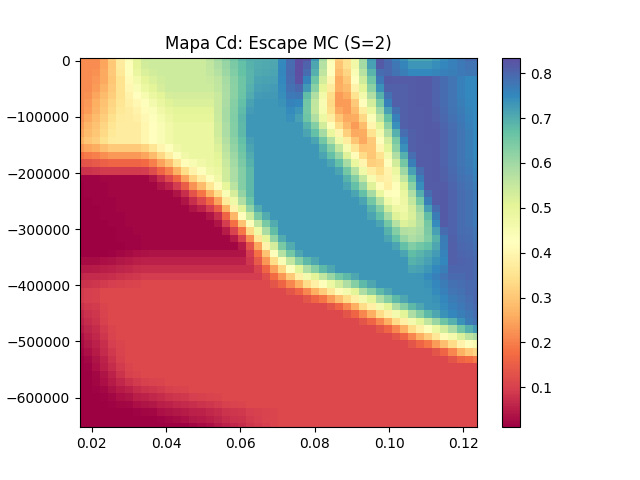
\includegraphics[width=\textwidth]{mapa_cd/mc_s2_mapa_esc.png}
        \caption{Puerto de escape}\label{fig:mapa_cd_escape}
    \end{subfigure}
    \caption{Mapas de $C_{D}$}\label{fig:mapa_cd_mc_s2}
\end{figure}

En el mapa del puerto de admisión se observa un máximo de $C_{D}\simeq 0.6$ para
para $l_{v}=62.95 mm$ y $\Delta P\simeq -7.37 kPa$, obteneniendo un flujo hacia
afuera del puerto de $\dot{0.122092} kg/seg$, este valor se obtiene para un
reflujo de gases residuales apenas abre el puerto de admisión, en particular
este valor se obtuvo para el el $10^{\circ}$ a 7000 RPM.
%
Las líneas de flujo para este caso se ven en la figura~\ref{fig:adm_cd_max}.
%
El menor valor también se obtiene para un valor muy próximo a la apertura del
puerto de admisión, siendo $C_{D}\simeq 0.12$ con un reflujo de
$\dot{m}\le 0.005$, $l_{v}=144.3 mm$ y $\Delta_{P}=-6.57 kPa$ para el puerto a
$590^{\circ}$ a 1000 RPM, las líneas de corriente para la flujometría de este
caso se ven en la figura~\ref{fig:adm_cd_min}.
%
En términos de flujo másico, el mayor valor  es de $\dot{m}=70 g/seg$ se da
durante un período de máxima apertura del puerto con $l_{v}=81.94 mm$ y
$\Delta_{P}=4.95 kPa$ siendo $C_{D}=0.32874$, la flujometría correspondiente se
ve en la figura~\ref{fig:adm_m_max}.

\begin{figure}[ht]
    \centering
    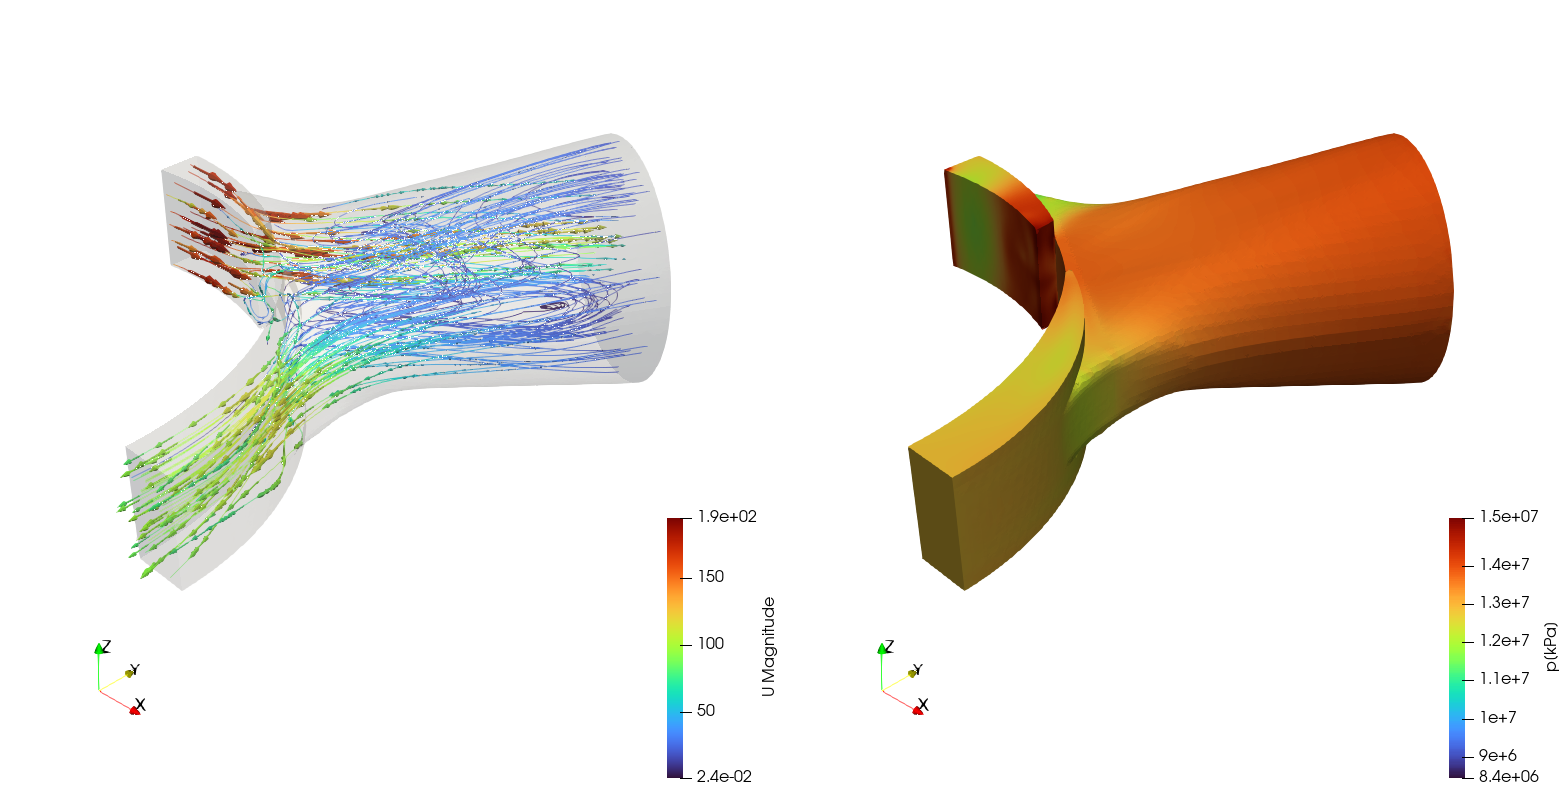
\includegraphics[width=0.7\textwidth]{flujometrias/adm_cd_max.png}
    \caption{Valor máximo de $C_{D}$}\label{fig:adm_cd_max}
\end{figure}

\begin{figure}[ht]
    \centering
    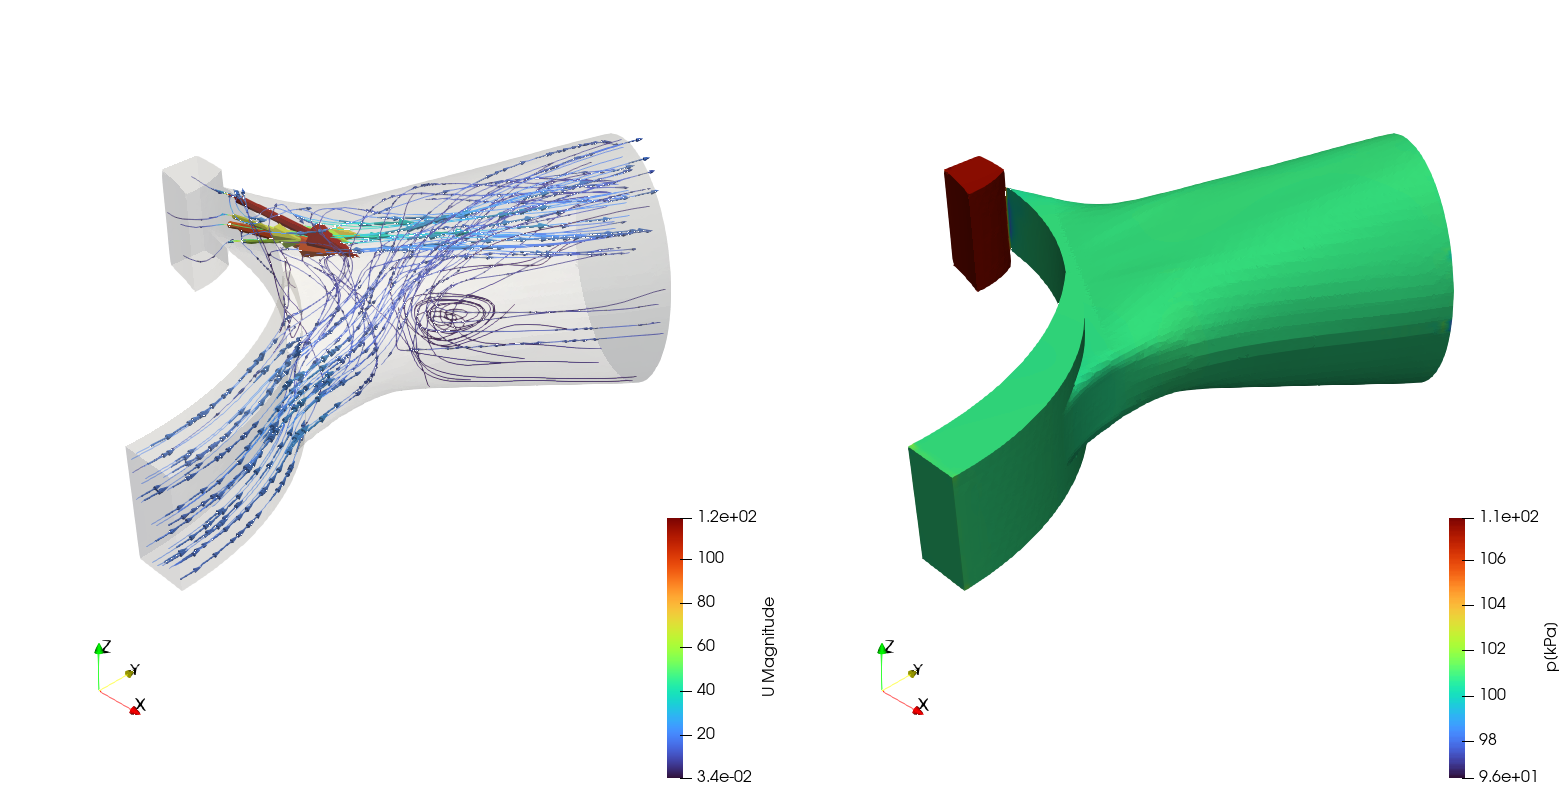
\includegraphics[width=0.7\textwidth]{flujometrias/adm_cd_min.png}
    \caption{Valor mínimo de $C_{D}$}\label{fig:adm_cd_min}
\end{figure}

\begin{figure}[ht]
    \centering
    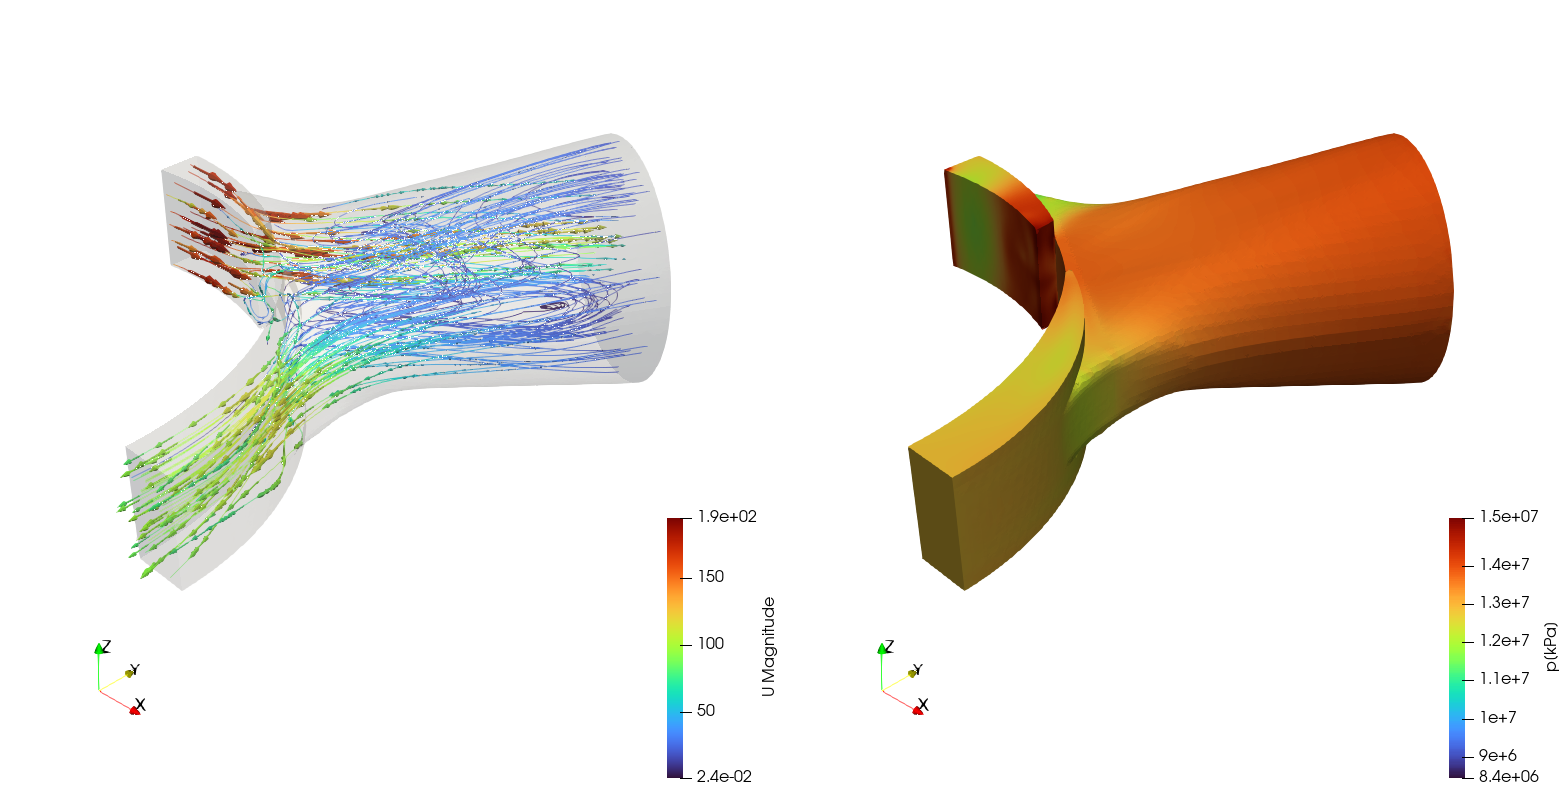
\includegraphics[width=0.7\textwidth]{flujometrias/adm_cd_max.png}
    \caption{Valor máximo de $\dot{m}$}\label{fig:adm_m_max}
\end{figure}

Para el puerto de escape se observa el máximo $C_{D}=0.57686$ para
$l_{v}=87.76 mm$, $\Delta_{P}=-10.7 kPa$ con un flujo másico de $145 g/s$
hacia afuera para $440^{\circ}$ a 9000 RPM.
%
Las líneas de corriente para este caso se muestran en la
figura~\ref{fig:esc_cd_max}.
%
El menor del mapa es de $C_{D}=0.09631$ para $l_{v}=16.83 mm$ y
$\Delta_{P}=-652.9 kPa$, un caso en el que se observa el flujo bloqueado por la
alta diferencia de presiones alcanzando un flujo másico de $\dot{m}=38,6 g/seg$,
en la figura~\ref{fig:esc_cd_min} se muestran las líneas de corriente para este caso.
%
El máximo valor de flujo másico se estima en $\dot{m}=176.1 g/seg$ para
$l_{v}=87.76 mm$ y $\Delta_{P}=-334 kPa$, esto con el ciclo a $440^{\circ}$ y 7000
RPM, los resultados de la flujometría se muestran en la figura~\ref{fig:esc_m_max}.

\begin{figure}[ht]
    \centering
    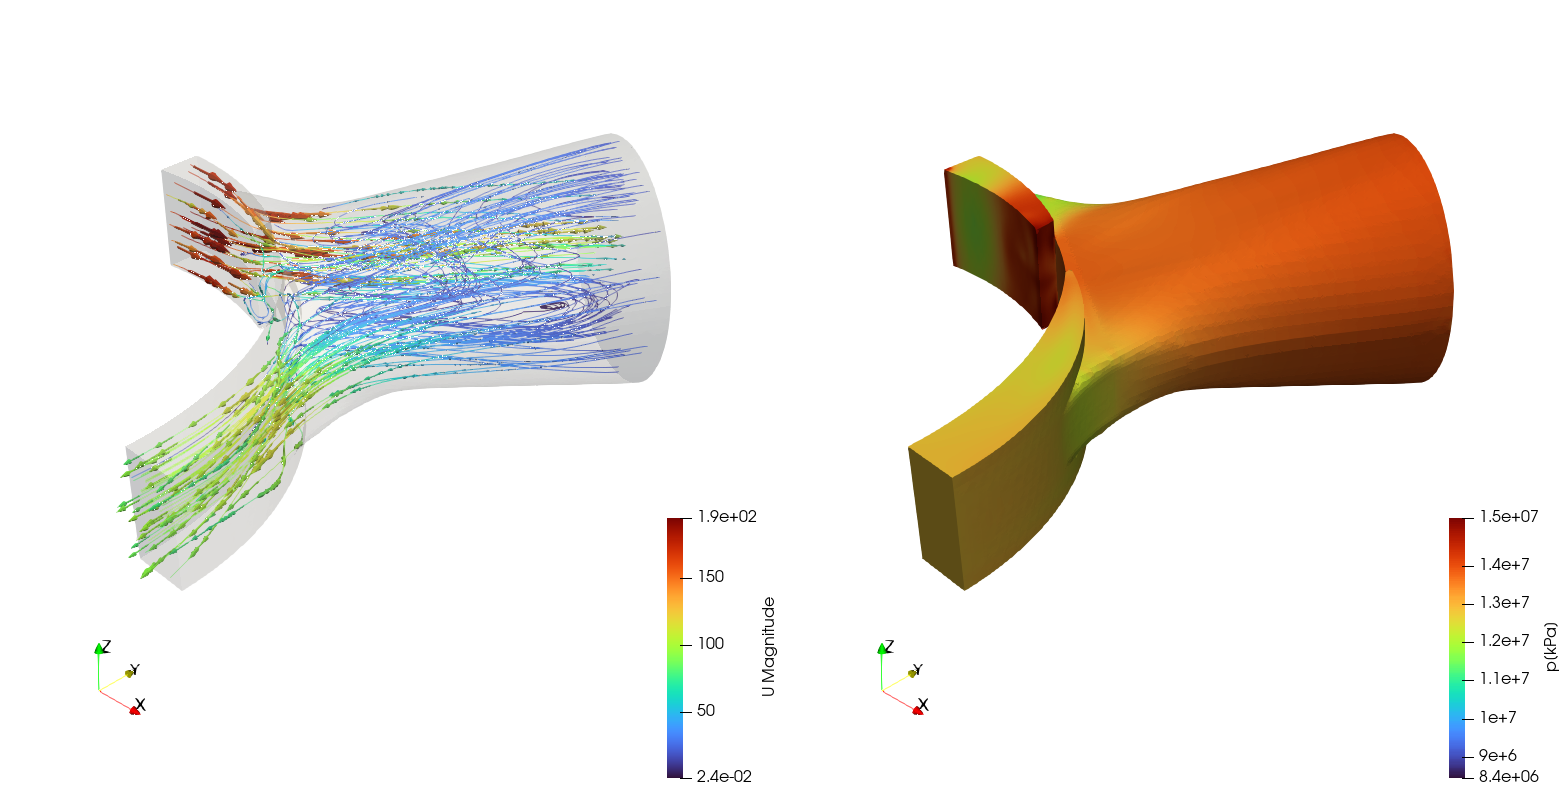
\includegraphics[width=0.7\textwidth]{flujometrias/adm_cd_max.png}
    \caption{Valor máximo de $C_{D}$}\label{fig:esc_cd_max}
\end{figure}

\begin{figure}[ht]
    \centering
    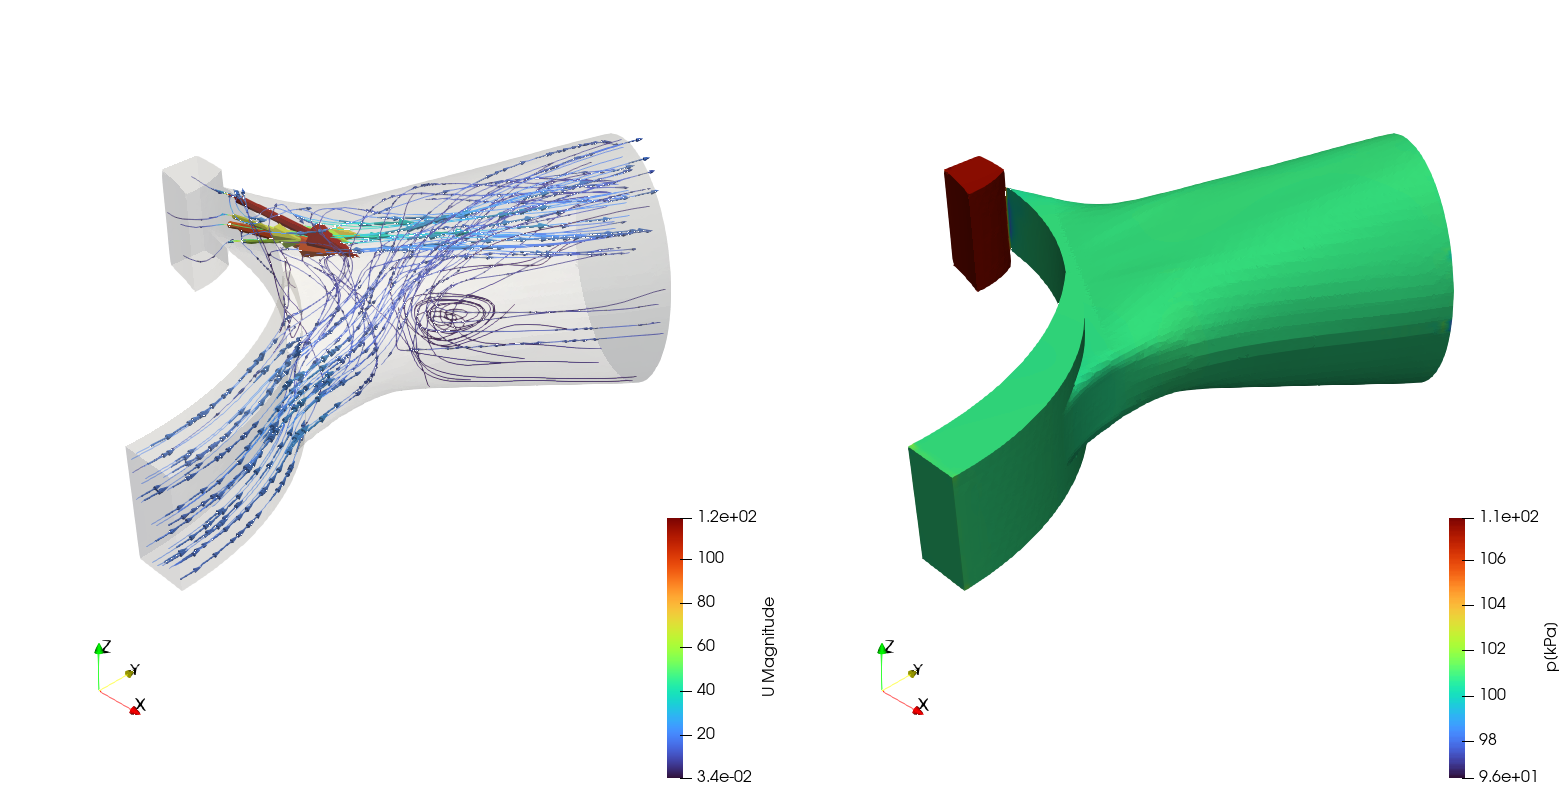
\includegraphics[width=0.7\textwidth]{flujometrias/adm_cd_min.png}
    \caption{Valor mínimo de $C_{D}$}\label{fig:esc_cd_min}
\end{figure}

\begin{figure}[ht]
    \centering
    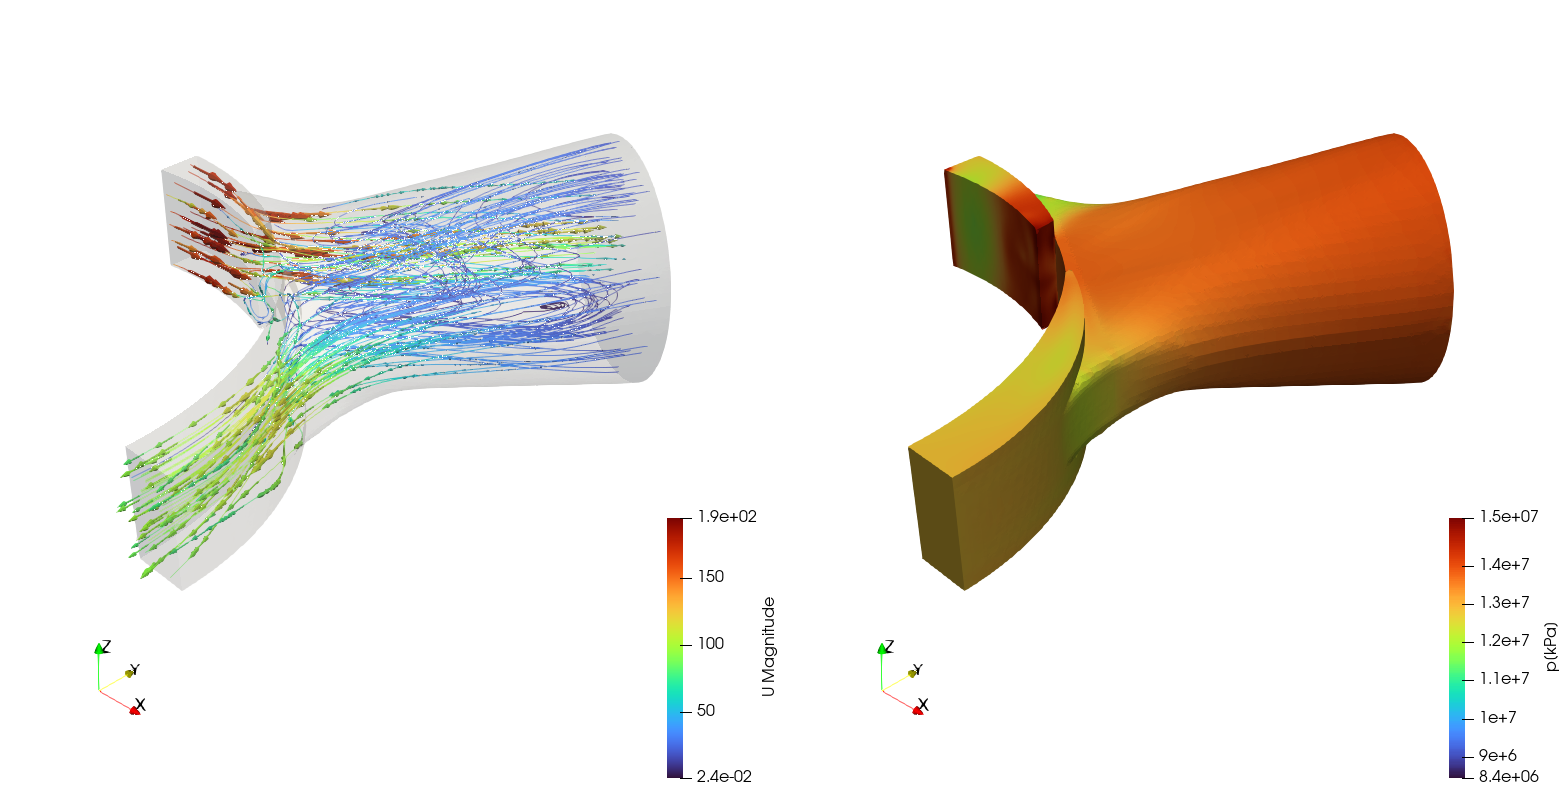
\includegraphics[width=0.7\textwidth]{flujometrias/adm_cd_max.png}
    \caption{Valor máximo de $\dot{m}$}\label{fig:esc_m_max}
\end{figure}

\begin{table}
  \centering
    \begin{tabular}{cccc} \toprule
      Caso  & lv        & $\Delta P$    & $C_{D}$   \\ \midrule
      0     & 0.016826  & -100331.39    &  0.213882 \\
      0     & 0.106775  & 5723.72       &  0.489375 \\
      0     & 0.016826  & -263797.72    &  0.011021 \\
      0     & 0.106775  & -3296.18      &  0.803197 \\
      0     & 0.016826  & -652902.78    &  0.011106 \\
      0     & 0.106775  & -9613.29      &  0.815804 \\
      0     & 0.016826  & -513568.73    &  0.011280 \\
      0     & 0.106775  & -3232.97      &  0.813186 \\
      1     & 0.026960  & -116996.12    &  0.375219 \\
      1     & 0.096641  & -3643.9       &  0.878414 \\
      1     & 0.026960  & -237724.11    &  0.018632 \\
      1     & 0.096641  & -6684.11      &  0.867774 \\
      1     &  0.02696  & -496509.46    &  0.111212 \\
      1     &  0.09664  & -18256.20     &  0.805830 \\
      1     & 0.026960  & -237724.11    &  0.022716 \\
      1     & 0.096641  & -6684.11      &  0.862647 \\
      2     & 0.047228  & -49343.47     &  0.541857 \\
      2     & 0.076373  & -5712.86      &  0.918061 \\
      2     & 0.047228  & -109348.67    &  0.487137 \\
      2     & 0.076373  & -17090.38     &  0.914182 \\
      3     & 0.067496  & 13.83         &  0.696967 \\
      3     & 0.071759  & -134.24       &  0.707263 \\
      3     & 0.067496  & -100073.52    &  0.731100 \\
      3     & 0.071759  & -24077.34     &  0.723965 \\
      4     & 0.075750  & -11793.31     &  0.946392 \\
      4     & 0.087764  & -33418.12     &  0.235717 \\
      4     & 0.087764  & -10715.70     &  0.221632 \\
      4     & 0.075750  & -5167.81      &  0.897169 \\
      6     & 0.123601  & -73.94        &  0.878522 \\ \bottomrule
    \end{tabular}
  \caption{Mapa de $C_D$ del puerto de escape} \label{tab:mapa_cd_escape}
\end{table}

\begin{table}
  \centering
  \begin{tabular}{cccc} \toprule
      Caso  & lv        & $\Delta P$    & $C_{D}$   \\ \midrule
      0     & 0.014432  & -6574.97      &  0.206543 \\
      0     & 0.081937  & -87.24        &  0.828822 \\
      0     & 0.014432  & 21856.29      &  0.243975 \\
      0     & 0.081937  & -573.65       &  0.738459 \\
      0     & 0.014432  & -19738.67     &  0.222406 \\
      0     & 0.081937  & 519.60        &  0.487115 \\
      0     & 0.081937  & 1571.95       &  0.587277 \\
      0     & 0.014432  & 18077.97      &  0.256415 \\
      0     & 0.014432  & 2668.61       &  0.247292 \\
      0     & 0.081937  & 0.98          &  0.025970 \\
      2     & 0.062951  & -297.79       &  0.816487 \\
      2     & 0.081937  & 292.92        &  0.466147 \\
      2     & 0.062951  & -7374.88      &  0.980617 \\
      2     & 0.081937  & 4953.85       &  0.541619 \\
      3     & 0.071763  & 4092.13       &  0.501641 \\
      3     & 0.025832  & -3689.81      &  0.289852 \\
      4     & 0.069767  & -789.00       &  0.615690 \\
      4     & 0.069767  & 7869.92       &  0.599348 \\
      4     & 0.005564  & -12539.15     &  0.534555 \\
      4     & 0.005564  & -10091.84     &  0.583979 \\ \bottomrule
    \end{tabular}
  \caption{Mapa de $C_d$ del puerto de Admisión} \label{tab:mapa_cd_admision}
\end{table}


La geometría obtenida luego de realizar la optimización con los mapas de $C_D$
incorporados a la simulación de ICESym se muestra en la figura \ref{fig:geom_nueva}.
%
Se puede ver que la geometría es similar a la inicial, siendo el puerto de
admisión algo menor en cuanto a diámetro que en el caso inicial.

Como es de esperarse, incorporar estos mapa al modelo del motor tiene un efecto
en el comportamiento del mismo, esto se puede observar principalmente en las
curvas de presión del motor.

% \subsection{Mapa de $C_D$}
%
Para obtener el mapa se tomaran valores de flujo másico en las combinaciones de
$(\Delta P, l_v)$ que están indicadas en la tabla~\ref{tab:casos}.
%
% En la figura \ref{fig:flujometrias} se ve que se eligieron más cantidad de
% muestreos en las zonas donde hay mayores cambios de presión.
%
% La figura \ref{fig:flujometrias} fué obtenida a partir de los resultados del
% simulador ICESym, restando para las velocidades seleccionadas la presión de la
% cámara a la presión en la boca del puerto.

\begin{figure}
    \centering
    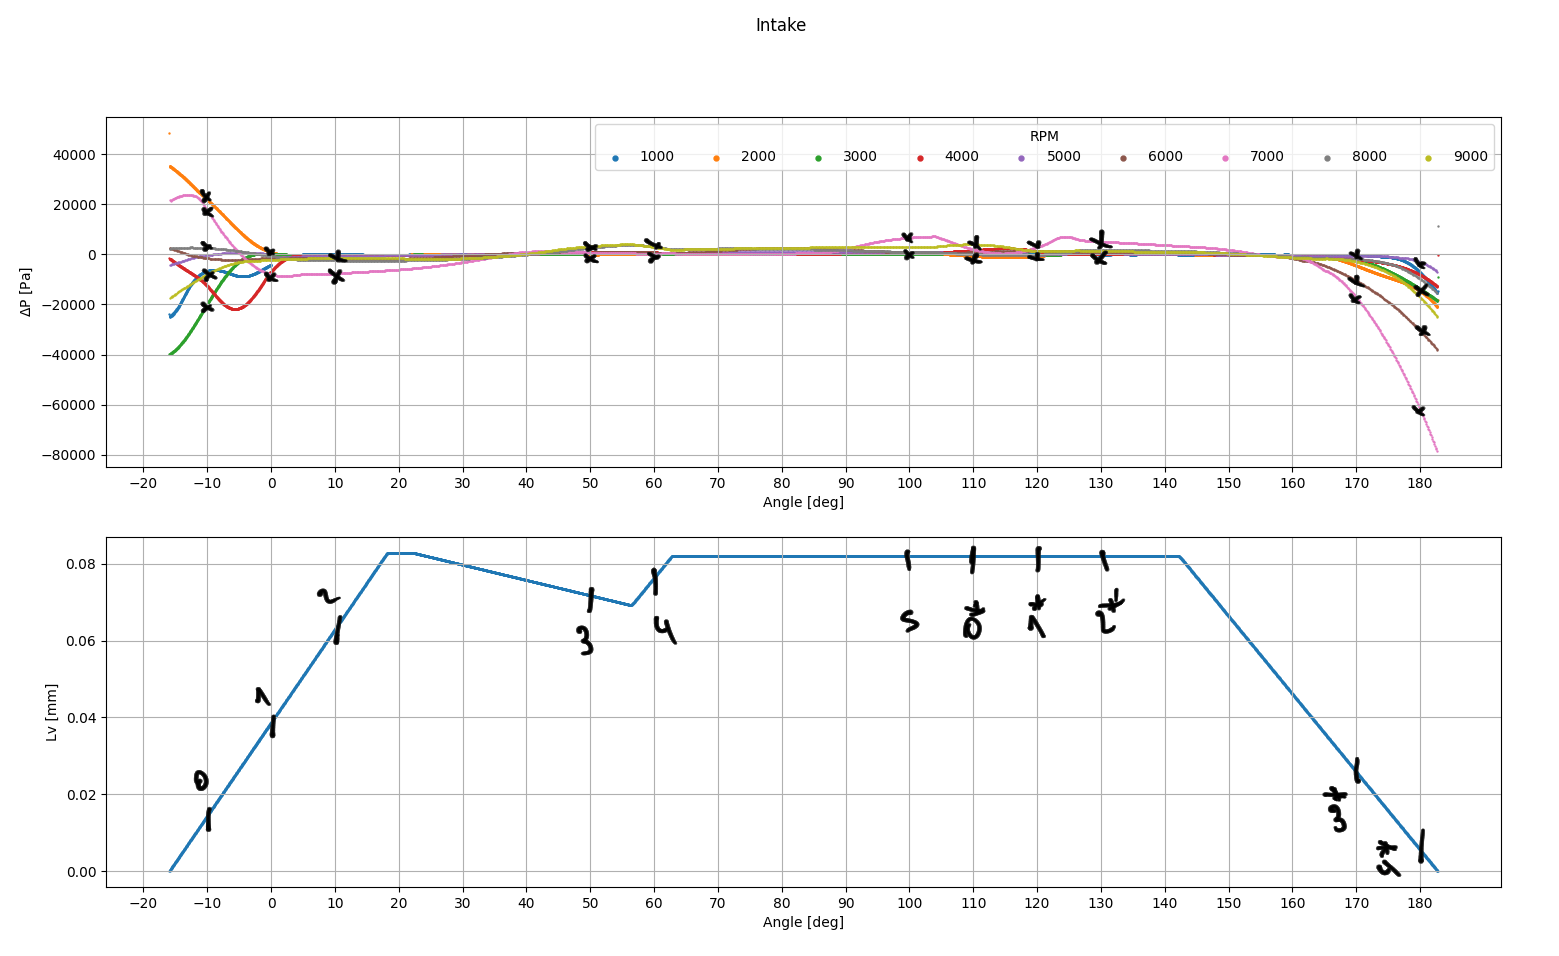
\includegraphics[width=1\textwidth]{flujometrias_admision.png}
    \caption{Flujometrías para el puerto de Admisión}\label{fig:flujometrias}
\end{figure}

\begin{table}
    \centering
    \begin{tabular}{rll} \toprule
        Caso & Ángulos  & Velocidades (rpm) \\ \midrule
        0    & -10, 110 & 1000, 2000, 3000, 7000, 8000 \\
        1    & 0, 120   & 2000, 7000 \\
        2    & 10, 130  & 2000, 7000 \\
        3    & 50, 170  & 3000, 7000, 9000 \\
        4    & 60, 180  & 3000, 5000, 6000, 7000 \\
        5    & 95       & 1000, 7000\\ \bottomrule
    \end{tabular}
    \caption{Flujometrías a realizar}\label{tab:casos}
\end{table}

Como se ve en la Figura~\ref{fig:flujometrias}, los puntos a evaluar son los
listados en la Tabla~\ref{tab:casos}.



\begin{figure}[h]
    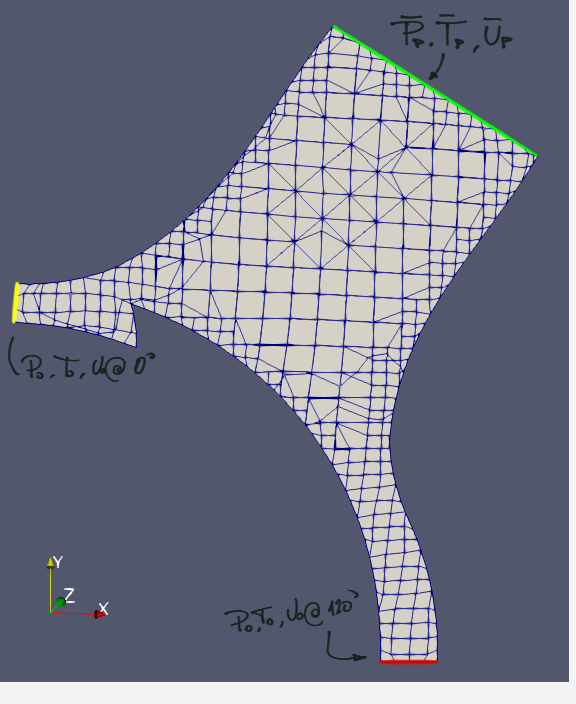
\includegraphics[width=0.8\textwidth]{caso_1-cc.png}
    \caption{Condiciones de borde}\label{fig:geom}
\end{figure}

Dentro del volumen de control, el campo de presiones se inicializa con el valor
medio de presiones de las cámaras y el campo de velocidades se hace
inicialmente (0,0,0).
%
El mapa de $C_D$ obetnido a partir de las flujoemtrías se lista en la
tabla~\ref{tab:mapaAdm} y~\ref{tab:mapaEsc} para los mapas de admisión y escape
respectivamente.


\begin{table}
  \parbox{.45\linewidth}{
  \centering
  \begin{tabular}{rccc}\toprule
    Item & $L_v[m]$ & $\Delta P[Pa]$ & $C_D$ \\ \midrule
    \lua{tex.print(mapaCd(myData.admision))}
    \bottomrule
    \end{tabular}
  \caption{Mapa $C_D$ del puerto de Admisión}\label{tab:mapaAdm}
  }
\hfill
\parbox{.45\linewidth}{
  \centering
  \begin{tabular}{rccc}\toprule
    Item & $L_v[m]$ & $\Delta P[Pa]$ & $C_D$ \\ \midrule
    \lua{tex.print(mapaCd(myData.escape))}
    \bottomrule
    \end{tabular}
  \caption{Mapa $C_D$ del puerto de Escape}\label{tab:mapaEsc}
}
\end{table}
